In this section, we describe the measurement model for a single-pixel
time-of-flight lidar sensor under diffuse, pulsed laser illumination. 
\subsection{Measurement Model}
Consider a laser which emits a pulse at time $t = 0$ with time-varying intensity
$g(t)$ uniformly illuminating some 3D scene. We parameterize the geometry of the
scene as a height map $z(x, y)$.
Neglecting albedo and falloff effects, an ideal detector counting photon events
from a location $(x,y)$ in the time interval $(n\Delta t, (n+1) \Delta t)$ would record

\begin{equation}
  \lambda_{x,y}[n] = \int_{n\Delta t}^{(n+1) \Delta t} (f * g)\paren*{t - 2z(x,y)/c} dt \label{single_loc_spad} 
\end{equation}  

where $c$ is the speed of light, and $f$ is a function that models the temporal uncertainty in the
detector. Single-photon avalanche diodes (SPADs) are highly sensitive
photodetectors which are able to record single photon events with high temporal
precision \cite{Stuff}. Since the detection of each photon can be described with
a Bernoulli random variable,
the total number of accumulated photons in this time interval follows a Poisson
distribution according to

\begin{equation}
  h[n] \sim \mathcal{P}\paren*{\sum_{x,y}\alpha_{x,y}\eta \lambda_{x,y}[n] + b} \label{global_hints}
\end{equation}

where $\alpha_{x,y} = r_{x,y}/z(x,y)^2$ captures the attenuation of the
photon counts due to the reflectance $r(x,y)$ of the scene and due to the
inverse square falloff $1/z(x,y)^2$.
In addition, $\eta$ is the detection probability of a photon
triggering a SPAD event, and $b = \eta a + d$ is the average number of background detections resulting
from ambient photons $a$
and erroneous ``dark count'' events $d$ resulting from noise within the SPAD.
\newpage
\begin{table*}[htbp]
  \begin{center}
    \begin{tabularx}{\linewidth}{*{2}{X}}
      \includegraphics[width=\textwidth/2-5pt]{sections/figures/spad_example/rgb.png} &
      \includegraphics[width=\textwidth/2-5pt]{sections/figures/spad_example/rawdepth.png} \\
      \includegraphics[width=\textwidth/2-5pt]{sections/figures/spad_example/depth_hist.png} &
      \includegraphics[width=\textwidth/2-5pt]{sections/figures/spad_example/spad_hist.png} \\
    \end{tabularx}
  \end{center}
  \caption{Sample Image. Top Left is the RGB image. Top Right is ground truth
    depth. Bottom Left is Raw ground truth depth histogram. Bottom Right is
    simulated SPAD measurements. Notice how closer depths are magnified and far
    depths are attenuated.}
\end{table*}

\subsection{Monocular depth estimation with global depth hints}
Given a single RGB image $I(x,y)$ and a vector of photon arrivals $h[n]$
described by equation \ref{global_hints}, we seek to
reconstruct the ground truth depth map $z(x,y)$.
Our method has two parts. First, we initialize our estimate of the depth map from the single RGB
image via a monocular depth estimator described below. Second, we refine this depth map using
the captured measurements $h[n]$ via a process we call Differentiable Histogram
Matching (DHM).
Differentiable histogram matching is a tool for post-processing the image to
match the depth map to the statistics we capture from the SPAD.

\paragraph{Initialization via CNN}
Convoluational Neural Networks have become increasingly capable of leveraging
monocular depth cues to produce accurate estimates of depth
from only a single image. We therefore choose to initialize our depth map
estimate $\hat z^{(0)}(x,y)$ using
a CNN. However, any depth estimator reliant on only a single
view will be unable to resolve the inherent scale ambiguity in the scene resulting
from the tradeoff between size of and distance to an object. The next step,
differentiable histogram matching, will resolve this ambiguity using the depth
information present in the SPAD histogram.

\paragraph{SPAD Denoising}
\begin{itemize}
  \item Discuss MLE for SPAD denoising
  \item Write optimization problem for SPAD denoising
  \item Show performance on a few examples 
\end{itemize}
\paragraph{Exact Histogram Matching}
\begin{figure}
  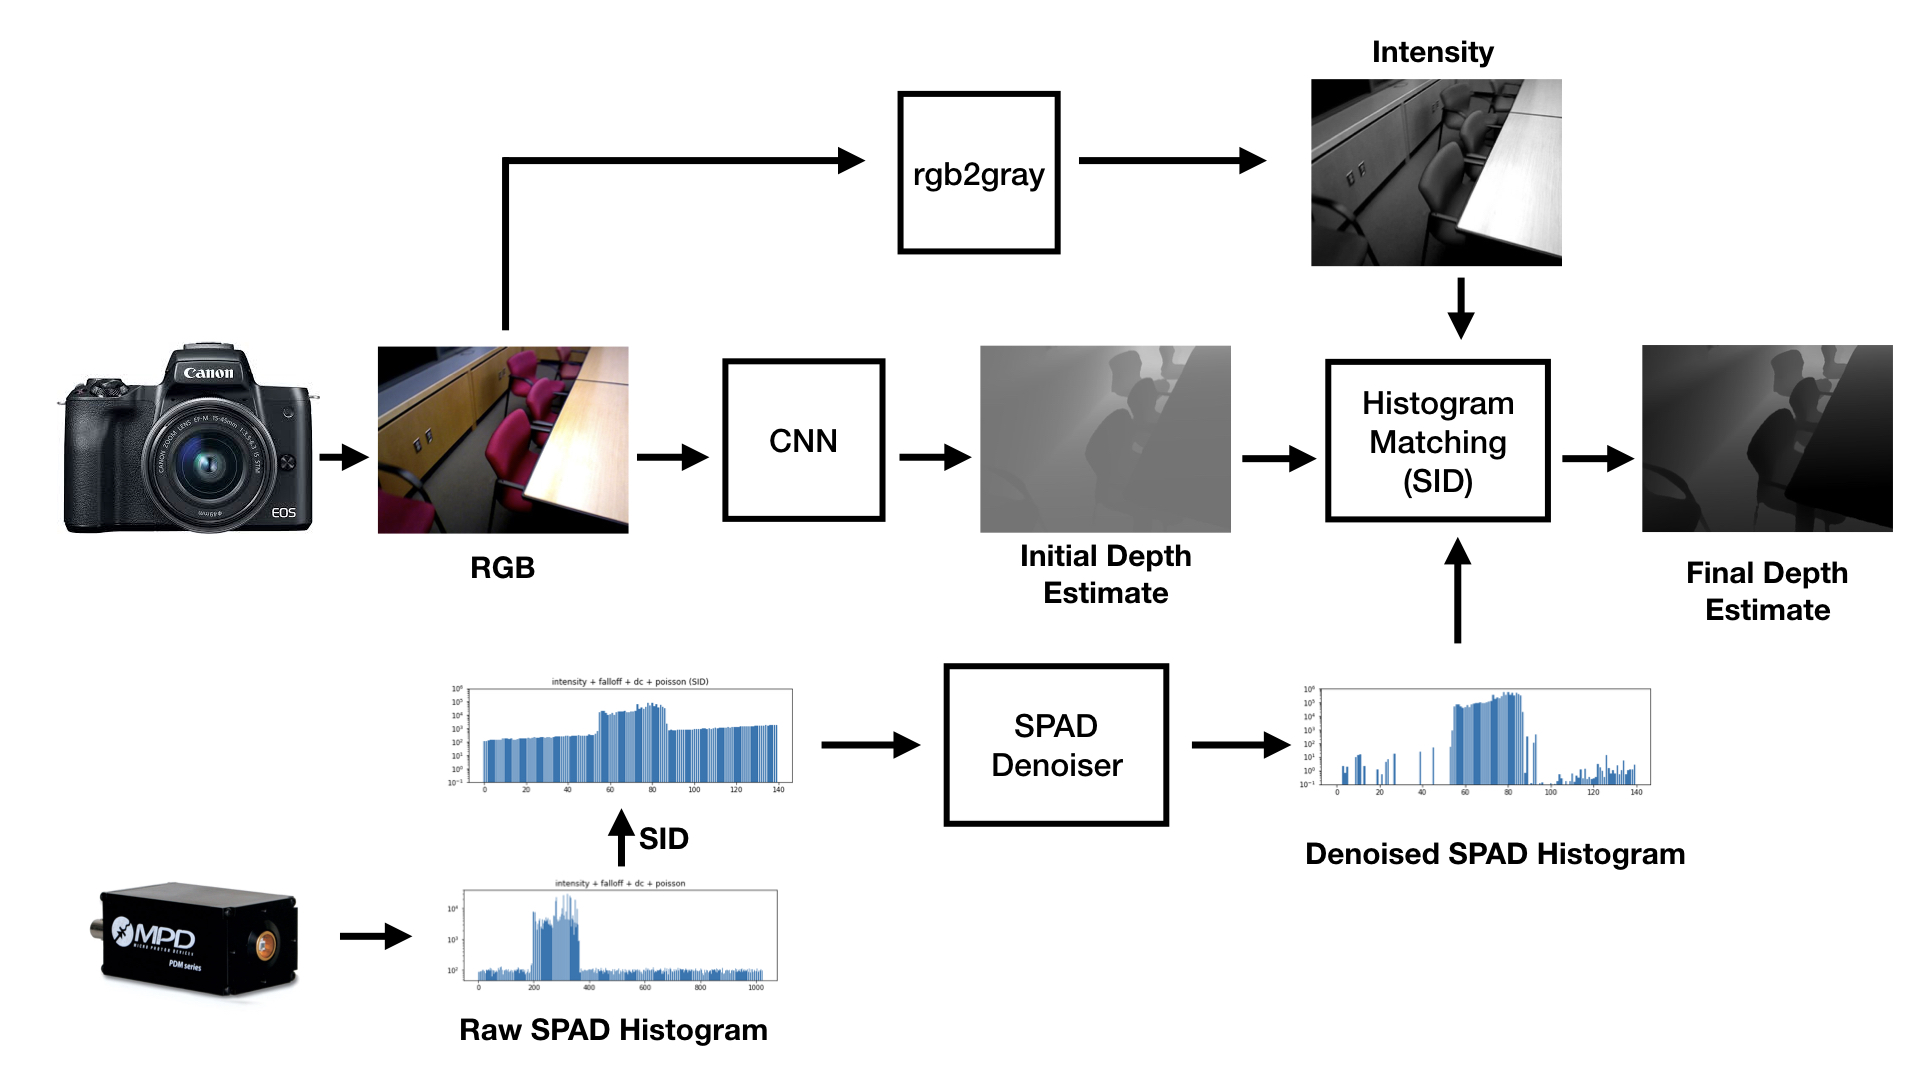
\includegraphics[width=\textwidth/2]{sections/figures/full_pipeline/full_pipeline.jpeg}
  \caption{\textbf{Overview of the full pipeline} We use a CNN to get an initial
  per-pixel depth estimate. We then perform gradient descent to optimize that
  estimate using the SPAD forward model and the dual-Sinkhorn distance
  .}
\end{figure}
An image's \textit{histogram} is a pair of vectors $(h, b)$ where $h_i$ is the number of
pixels of the image whose value lies in the range $[b_i, b_i+1)$.
Then, given a source image $S$ with histogram $(h_s, b)$ and a target histogram
$(h_t, b)$, histogram matching generates a new image $M$ such that $h_m \approx
h_t$ and the pixel values in $M$ are in the same relative order as in $S$.


\subsection{Implementation Details}
For the Monocular Depth Estimator, we use pretrained versions of the
the Deep Ordinal Regression Network (DORN) \cite{} and the DenseDepth Network.
The exact histogram matching method is as described in \cite{}.


